%% LAB 4:Introduction to Latex and GraphViz
%%%%%%%%%%%%%%%%%%%%%%%%%%%%%%%%%%%%%%%%%%%%%%%%%%%%%%%%%%%%%

\documentclass[11pt,a4paper]{amsart}


\usepackage{amsmath}%
\usepackage{amsfonts}%
\usepackage{amssymb}%
\usepackage{graphicx}
\usepackage{hyperref}
\usepackage[left=2.00cm, right=2.00cm, top=2.00cm, bottom=2.00cm]{geometry}

%------------------------------------------------------------
% Theorem like environments
%
\newtheorem{theorem}{Theorem}
\theoremstyle{plain}
\newtheorem{acknowledgement}{Acknowledgment}
\newtheorem{algorithm}{Algorithm}
\newtheorem{axiom}{Axiom}
\newtheorem{case}{Case}
\newtheorem{claim}{Claim}
\newtheorem{conclusion}{Conclusion}
\newtheorem{condition}{Condition}
\newtheorem{conjecture}{Conjecture}
\newtheorem{corollary}{Corollary}
\newtheorem{criterion}{Criterion}
\newtheorem{definition}{Definition}
\newtheorem{example}{Example}
\newtheorem{exercise}{Exercise}
\newtheorem{lemma}{Lemma}
\newtheorem{notation}{Notation}
\newtheorem{problem}{Problem}
\newtheorem{proposition}{Proposition}
\newtheorem{remark}{Remark}
\newtheorem{solution}{Solution}
\newtheorem{summary}{Summary}
\numberwithin{equation}{section}

\theoremstyle{definition}
\newtheorem{defn}{Definition}[section]
%--------------------------------------------------------

\begin{document}



\title{BINARY HEAPS}
\author{NIRAV PATEL (CS14M036)}

%\address{1^(st) Year M.Tech. CSE,IIT Madras.}
%\email{nirav111nirav@gmail.com}

\date{\today}


\begin{abstract}
This document is about Binary heaps.It explains ``Binary Heap and its operations".
\end{abstract}

\maketitle

\section{Introduction}

\begin{defn}
A \textbf{Binary heap} is a complete binary tree with the following properties:

1.\textbf{MIN-HEAP}: If every node has key value less than its children,then it is called Min-Heap.

2.\textbf{MAX-HEAP}: If every node has key value greater than its children,then it is called Max-Heap.

\end{defn}

\noindent \\Basically Binary heap is a \emph{Dictionary} data structure.It is also used as a \emph{priority queue} as the root of the binary heap will be either minimum or maximum of all elements depending whether it is min-heap or max-heap.

\noindent \\We will show example of max-heap using following example:

\begin{figure}[h] \label{fig:heap_example}
	\includegraphics[scale=0.5]{Heap_example.png}
	\caption{Example of binary max-heap}
\end{figure}


\noindent Figure \ref{fig:heap_example} gives the tree view of binary max-heap.We can see from the figure that the key value of every node in the tree is larger than the key values of its children.
Root is having the highest key value.

\section{Abstract Data Type}
Heap ADT contains following operations:
1.void Insert(ElementType)
2.ElementType ExtractMin();
3.void BuildHeap(ElementType[]);

\subsection{Subsection}
Subsection text.

\subsubsection{Subsubsection}
Subsubsection text.

\paragraph{Paragraph}
Paragraph text.

\subparagraph{Subparagraph}Subparagraph text.\vspace{2mm}

Select a part of the text then click on the button Emphasize (H!), or
Bold (Fs), or Italic (Kt), or Slanted (Kt) to typeset \emph{Emphasize},
\textbf{Bold}, \textit{Italics}, \textsl{Slanted} texts.

You can also typeset \textrm{Roman}, \textsf{Sans Serif}, \textsc{Small Caps},
and \texttt{Typewriter} texts.

You can also apply the special, mathematics only commands $\mathbb{BLACKBOARD}$
$\mathbb{BOLD}$, $\mathcal{CALLIGRAPHIC}$, and $\mathfrak{fraktur}$. Note that
blackboard bold and calligraphic are correct only when applied to uppercase
letters A through Z.

You can apply the size tags -- Format menu, Font size submenu -- {\tiny tiny},
{\scriptsize scriptsize}, {\footnotesize footnotesize}, {\small small},
{\normalsize normalsize}, {\large large}, {\Large Large}, {\LARGE LARGE},
{\huge huge} and {\Huge Huge}.

You can use the \verb"\begin{quote} etc. \end{quote}" environment for typesetting
short quotations. Select the text then click on Insert, Quotations, Short Quotations:

\begin{quote}
The buck stops here. \emph{Harry Truman}

Ask not what your country can do for you; ask what you can do for your
country. \emph{John F Kennedy}

I am not a crook. \emph{Richard Nixon}


\end{quote}

The Quotation environment is used for quotations of more than one paragraph. Following
is the beginning of \emph{The Jungle Books} by Rudyard Kipling. (You should select
the text first then click on Insert, Quotations, Quotation):

\begin{quotation}
It was seven o'clock of a very warm evening in the Seeonee Hills when Father Wolf woke
up from his day's rest, scratched himself, yawned  and spread out his paws one after
the other to get rid of sleepy feeling in their tips. Mother Wolf lay with her big gray
nose dropped across her four tumbling, squealing cubs, and the moon shone into the
mouth of the cave where they all lived. ``\emph{Augrh}'' said Father Wolf, ``it is time
to hunt again.'' And he was going to spring down hill when a little shadow with a bushy
tail crossed the threshold and whined: ``Good luck go with you, O Chief of the Wolves;
and good luck and strong white teeth go with the noble children, that they may never
forget the hungry in this world.''

It was the jackal---Tabaqui the Dish-licker---and the wolves of India despise Tabaqui
because he runs about making mischief, and telling tales, and eating rags and pieces of
leather from the village rubbish-heaps. But they are afraid of him too, because
Tabaqui, more than any one else in the jungle, is apt to go mad, and then he forgets
that he was afraid of anyone, and runs through the forest biting everything in his way.
\end{quotation}

Use the Verbatim environment if you want \LaTeX\ to preserve spacing, perhaps when
including a fragment from a program such as:
\begin{verbatim}
#include <iostream>         // < > is used for standard libraries.
void main(void)             // ''main'' method always called first.
{
 cout << ''This is a message.'';
                            // Send to output stream.
}
\end{verbatim}
(After selecting the text click on Insert, Code Environments, Code.)


\subsection{Mathematics and Text}

It holds \cite{KarelRektorys} the following
\begin{theorem}
(The Currant minimax principle.) Let $T$ be completely continuous selfadjoint operator
in a Hilbert space $H$. Let $n$ be an arbitrary integer and let $u_1,\ldots,u_{n-1}$ be
an arbitrary system of $n-1$ linearly independent elements of $H$. Denote
\begin{equation}
\max_{\substack{v\in H, v\neq0\\
(v,u_1)=0,\ldots,(v,u_n)=0}}
\frac{(Tv,v)}{(v,v)}=m(u_1,\ldots, u_{n-1}) \label{eqn10}
\end{equation}


Then the $n$-th eigenvalue of $T$ is equal to the minimum of these maxima, when minimizing over all linearly independent systems $u_1,\ldots u_{n-1}$ in $H$,
\begin{equation}
\mu_n = \min_{\substack{u_1,\ldots, u_{n-1}\in H}} m(u_1,\ldots, u_{n-1}) \label{eqn20}
\end{equation}
\end{theorem}
The above equations are automatically numbered as equation (\ref{eqn10}) and
(\ref{eqn20}).

\subsection{List Environments}

You can create numbered, bulleted, and description lists
(Use the Itemization or Enumeration buttons, or click on the Insert menu
then chose an item from the Enumeration submenu):

\begin{enumerate}
\item List item 1

\item List item 2

	\begin{enumerate}
	\item A list item under a list item.

	However, the typeset style for this level is different.

	\item Just another list item under a list item.

		\begin{enumerate}
		\item Third level list item under a list item.

			\begin{enumerate}
			\item Fourth and final level of list items allowed.
			\end{enumerate}
		\end{enumerate}
	\end{enumerate}
\end{enumerate}

\begin{itemize}
\item Bullet item 1

\item Bullet item 2

		\begin{itemize}
		\item Second level bullet item.

			\begin{itemize}
			\item Third level bullet item.

				\begin{itemize}
				\item Fourth (and final) level bullet item.
				\end{itemize}
			\end{itemize}
		\end{itemize}
\end{itemize}

\begin{description}
\item[Description List] Each description list item has a term followed by the
description of that term. Double click the term box to enter the term, or to
change it.

\item[Bunyip] Mythical beast of Australian Aboriginal legends.
\end{description}

\subsection{Theorem-like Environments}

The following theorem-like environments (in alphabetical order) are available
in this style.

\begin{acknowledgement}
This is an acknowledgement
\end{acknowledgement}

\begin{algorithm}
This is an algorithm
\end{algorithm}

\begin{axiom}
This is an axiom
\end{axiom}

\begin{case}
This is a case
\end{case}

\begin{claim}
This is a claim
\end{claim}

\begin{conclusion}
This is a conclusion
\end{conclusion}

\begin{condition}
This is a condition
\end{condition}

\begin{conjecture}
This is a conjecture
\end{conjecture}

\begin{corollary}
This is a corollary
\end{corollary}

\begin{criterion}
This is a criterion
\end{criterion}

\begin{definition}
This is a definition
\end{definition}

\begin{example}
This is an example
\end{example}

\begin{exercise}
This is an exercise
\end{exercise}

\begin{lemma}
This is a lemma
\end{lemma}


\begin{notation}
This is notation
\end{notation}

\begin{problem}
This is a problem
\end{problem}

\begin{proposition}
This is a proposition
\end{proposition}

\begin{remark}
This is a remark
\end{remark}

\begin{solution}
This is a solution
\end{solution}

\begin{summary}
This is a summary
\end{summary}

\begin{theorem}
This is a theorem
\end{theorem}



\section{Figures and Graphviz}

We have included the following three ``.gv'' files as samples. Many more can be found in graphviz website.
\begin{enumerate}
	\item {\tt graph1.gv}
	\item {\tt graph2.gv} and
	\item {\tt profile.gv}
\end{enumerate}

These ``.gv'' files can be processed by a variety of tools included in the graphviz package. I used the ``dot'' tool (see \url{http://www.graphviz.org/pdf/dotguide.pdf}) to generate the figures in pdf and png formats. You can generate them in several other formats as well.

\begin{figure}[h] \label{fig:pdf}
	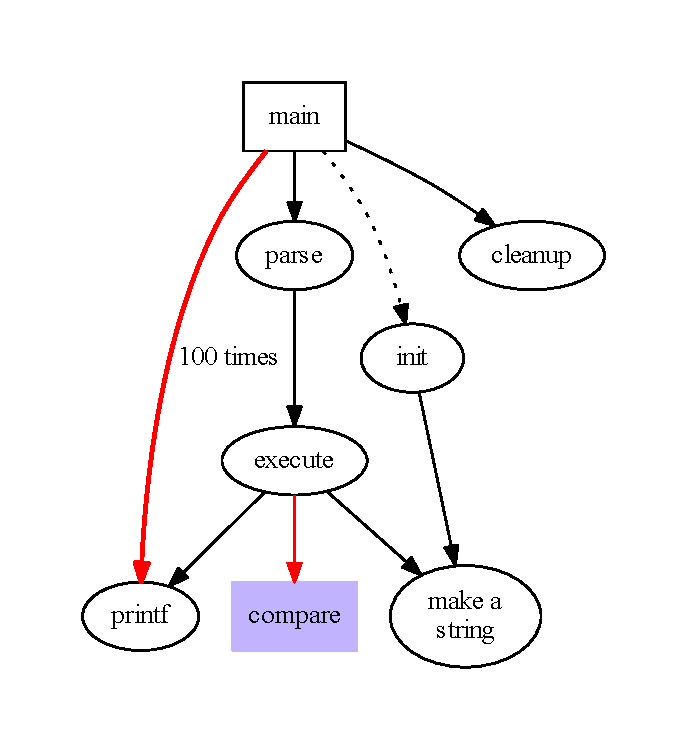
\includegraphics[scale=0.5]{graph1.pdf} \hspace{0.5in}
	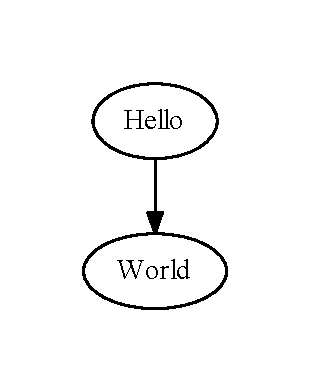
\includegraphics[scale=1]{graph2.pdf}
	\caption{Illustrates how you can include PDF figures.}
	
\end{figure}


\begin{figure}[h] \label{fig:png}
	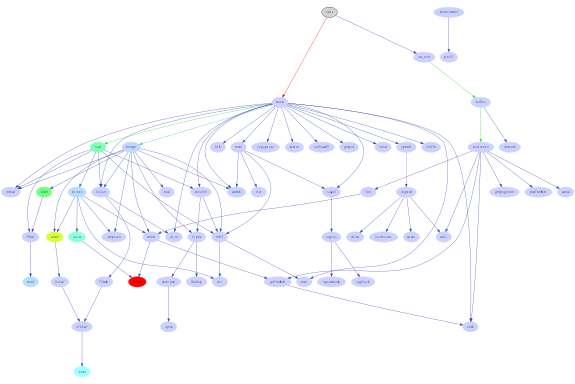
\includegraphics[scale=0.7]{profile.png} \hspace{0.5in}
	\caption{Illustrates how you can include a png figure.}
	
\end{figure}

Figures~\ref{fig:pdf} and \ref{fig:png} illustrate how the figures can be included into the tex file. 

This text is a sample for a short bibliography. You can cite a book by making use of
the command \verb"\cite{KarelRektorys}": \cite{KarelRektorys}. Papers can be cited
similarly: \cite{Bertoti97}. If you want multiple citations to appear in a single set
of square brackets you must type all of the citation keys inside a single citation,
separating each with a comma. Here is an example: \cite{Bertoti97, Szeidl2001,
Carlson67}.

\newpage

\begin{thebibliography}{9}                                                                                                %
\bibitem {KarelRektorys}Rektorys, K., \textit{Variational methods in Mathematics,
Science and Engineering}, D. Reidel Publishing Company,
Dordrecht-Hollanf/Boston-U.S.A., 2th edition, 1975

\bibitem {Bertoti97} \textsc{Bert\'{o}ti, E.}:\ \textit{On mixed variational formulation
of linear elasticity using nonsymmetric stresses and displacements}, International
Journal for Numerical Methods in Engineering., \textbf{42}, (1997), 561-578.

\bibitem {Szeidl2001} \textsc{Szeidl, G.}:\ \textit{Boundary integral equations for
plane problems in terms of stress functions of order one}, Journal of Computational and
Applied Mechanics, \textbf{2}(2), (2001), 237-261.

\bibitem {Carlson67}  \textsc{Carlson D. E.}:\ \textit{On G\"{u}nther's stress functions
for couple stresses}, Quart. Appl. Math., \textbf{25}, (1967), 139-146.
\end{thebibliography}
\end{document}
